%%%%%%%%%%%%%%%%%%%%%%%%%%%%%%%%%%%%%%%%%%
% Engineering problems / LaTeX Template
%		Semester 5
%		Institut d'Optique Graduate School
%%%%%%%%%%%%%%%%%%%%%%%%%%%%%%%%%%%%%%%%%%
%	5N-ONIP-Block1	/ Python for Science
%%%%%%%%%%%%%%%%%%%%%%%%%%%%%%%%%%%%%%%%%%
%
% Created by:
%	Julien VILLEMEJANE - 25/sep/2024
% Modified by:
%	
%
%%%%%%%%%%%%%%%%%%%%%%%%%%%%%%%%%%%%%%%%%%
% Professional Newsletter Template
% LaTeX Template
% Version 1.0 (09/03/14)
%
% Created by:
% Bob Kerstetter (https://www.tug.org/texshowcase/) and extensively modified by:
% Vel (vel@latextemplates.com)
% 
% This template has been downloaded from:
% http://www.LaTeXTemplates.com
%
% License:
% CC BY-NC-SA 3.0 (http://creativecommons.org/licenses/by-nc-sa/3.0/)
%
%%%%%%%%%%%%%%%%%%%%%%%%%%%%%%%%%%%%%%%%%

\documentclass[10pt]{article} % The default font size is 10pt; 11pt and 12pt are alternatives

%%%%%%%%%%%%%%%%%%%%%%%%%%%%%%%%%%%%%%%%%
% Professional Newsletter Template
% Structural Definitions File
% Version 1.0 (09/03/14)
%
% Created by:
% Vel (vel@latextemplates.com)
% 
% This file has been downloaded from:
% http://www.LaTeXTemplates.com
%
% License:
% CC BY-NC-SA 3.0 (http://creativecommons.org/licenses/by-nc-sa/3.0/)
%
%%%%%%%%%%%%%%%%%%%%%%%%%%%%%%%%%%%%%%%%%

%----------------------------------------------------------------------------------------
%	REQUIRED PACKAGES
%----------------------------------------------------------------------------------------

\usepackage{graphicx} % Required for including images
\usepackage{microtype} % Improved typography
\usepackage{multicol} % Used for the two-column layout of the document
\usepackage{booktabs} % Required for nice horizontal rules in tables
\usepackage{wrapfig} % Required for in-line images
\usepackage{float} % Required for forcing figures not to float with the [H] parameter

%------------------------------------------------
% Fonts

\usepackage{charter} % Use the Charter font as the main document font
\usepackage{courier} % Use the Courier font for \texttt (monospaced) only
\usepackage[T1]{fontenc} % Use T1 font encoding
\usepackage{lmodern}

%------------------------------------------------
% List Separation

\usepackage{enumitem} % Required to customize the list environments
\setlist{noitemsep,nolistsep} % Remove spacing before, after and within lists for a compact look

%------------------------------------------------
% Figure and Table Caption Styles

\usepackage{caption} % Required for changing caption styles
\captionsetup[table]{labelfont={bf,sf},labelsep=period,justification=justified} % Specify the table caption style
\captionsetup[figure]{labelfont={sf,bf},labelsep=period,justification=justified, font=small} % Specify the figure caption style
\setlength{\abovecaptionskip}{10pt} % Whitespace above captions

%------------------------------------------------
% Spacing Between Paragraphs

\makeatletter
\usepackage{parskip}
\setlength{\parskip}{6pt}
\newcommand{\@minipagerestore}{\setlength{\parskip}{6pt}}
\makeatother

%----------------------------------------------------------------------------------------
%	PAGE MARGINS AND SPACINGS
%----------------------------------------------------------------------------------------

\textwidth = 7 in % Text width
\textheight = 10 in % Text height
\oddsidemargin = -18pt % Left side margin on odd pages
\evensidemargin = -18pt % Left side margin on even pages
\topmargin = -36pt % Top margin
\headheight = 0pt % Remove the header by setting its space to 0
\headsep = 0pt % Remove the space between the header and top of the page
\parskip = 4pt % Space between paragraph
\parindent = 0.0in % Paragraph indentation
\pagestyle{empty} % Disable page numbering

%----------------------------------------------------------------------------------------
%	COLORS
%----------------------------------------------------------------------------------------

\usepackage[dvipsnames,svgnames]{xcolor} % Required to specify custom colors

\definecolor{altncolor}{rgb}{.8,0,0} % Dark red
%\definecolor{altncolor}{rgb}{.2,.4,.8} % Dark blue
%\definecolor{altncolor}{rgb}{.84,.16,.16} % Red

\usepackage[colorlinks=true, linkcolor=altncolor, anchorcolor=altncolor, citecolor=altncolor, filecolor=altncolor, menucolor=altncolor, urlcolor=altncolor]{hyperref} % Use the color defined above for all links

%----------------------------------------------------------------------------------------
%	DRAWINGS & CIRCUITS
%----------------------------------------------------------------------------------------

\usepackage{tikz}
\usepackage{pgfplots}

\usepackage[european, straightvoltages]{circuitikz}
\usetikzlibrary{babel, patterns, patterns.meta, calc}

%----------------------------------------------------------------------------------------
%	PDF
%----------------------------------------------------------------------------------------

\usepackage{pdfpages}

%----------------------------------------------------------------------------------------
%	BOX STYLES
%----------------------------------------------------------------------------------------

\usepackage[framemethod=TikZ]{mdframed}% Required for creating boxes
\mdfdefinestyle{sidebar}{
    linecolor=black, % Outer line color
    outerlinewidth=0.5pt, % Outer line width
    roundcorner=0pt, % Amount of corner rounding
    innertopmargin=10pt, % Top margin
    innerbottommargin=10pt, % Bottom margin
    innerrightmargin=10pt, % Right margin
    innerleftmargin=10pt, % Left margin
    backgroundcolor=white, % Box background color
    frametitlealignment=\centering,
    frametitlebackgroundcolor=gray!20, % Title background color
    frametitlerule=false, % Title rule - true or false
    frametitlerulecolor=white, % Title rule color
    frametitlerulewidth=0.5pt, % Title rule width
    frametitlefont=\Large\bfseries, % Title heading font specification
    font=\small
}

\mdfdefinestyle{intextbox}{
    linecolor=black, % Outer line color
    outerlinewidth=0.5pt, % Outer line width
    roundcorner=10pt, % Amount of corner rounding
    innertopmargin=7pt, % Top margin
    innerbottommargin=7pt, % Bottom margin
    innerrightmargin=7pt, % Right margin
    innerleftmargin=7pt, % Left margin
    backgroundcolor=white, % Box background color
    frametitlealignment=\centering,
    frametitlebackgroundcolor=gray!20, % Title background color
    frametitlerule=false, % Title rule - true or false
    frametitlerulecolor=white, % Title rule color
    frametitlerulewidth=0.5pt, % Title rule width
    frametitlefont=\Large\bfseries % Title heading font specification
}

\mdfdefinestyle{aavbox}{
    linecolor=black, % Outer line color
    outerlinewidth=0.2pt, % Outer line width
    roundcorner=5pt, % Amount of corner rounding
    innertopmargin=7pt, % Top margin
    innerbottommargin=7pt, % Bottom margin
    innerrightmargin=7pt, % Right margin
    innerleftmargin=7pt, % Left margin
    backgroundcolor=gray!10, % Box background color
    frametitlealignment=\centering,
    frametitlebackgroundcolor=gray!30, % Title background color
    frametitlerule=false, % Title rule - true or false
    frametitlerulecolor=white, % Title rule color
    frametitlerulewidth=0.2pt, % Title rule width
    frametitlefont=\Large\bfseries % Title heading font specification
}

%----------------------------------------------------------------------------------------
%	HEADING STYLE
%----------------------------------------------------------------------------------------

\newcommand{\heading}[2]{ % Define the \heading command
\vspace{#2} % White space above the heading
{\begin{center}\Large\textbf{#1}\end{center}} % The heading style
\vspace{#2} % White space below the heading
}

\newcommand{\BackToContents}{\hyperlink{contents}{{\small Back to Contents}}} % Define a command for linking back to the contents of the newsletter

\usepackage{listings}
\lstset{language = Python, 
	basicstyle={\small \color{black}}, 
	tabsize = 3,
	commentstyle=\color{black!70!green},
	linewidth=160mm,
	framexleftmargin=5mm, frame=shadowbox, rulesepcolor=\color{black},
  	numbers=left,
	xleftmargin=40pt,
	escapechar=|
} % Include the document which specifies all packages and structural customizations for this template
\usepackage{amsmath}

%----------------------------------------------------------------------------------------
%	DOCUMENT INFORMATIONS
%----------------------------------------------------------------------------------------
\def\module{Interfaçage Numérique}
\def\submodule{IntNum}
\def\moduleSmall{6N-047-SCI / IN}
\def\year{2024-2025}
\def\problem{TD Conversion Analogique Numérique}
\def\problemName{IntNum / TD Conversion Analogique Numérique}

\def\validation{}

\def\scheduleCM{0}
\def\scheduleTD{1}
\def\scheduleTDcomputer{0}
\def\scheduleTP{0}

\def\workingTeam{}

\def\workingSpecial{}

\def\keywords{Systèmes asservis;ALI;FFT}


\begin{document}
%----------------------------------------------------------------------------------------
%	HEADER IMAGE
%----------------------------------------------------------------------------------------

\begin{figure}[h!]
\centering
\includegraphics[width=0.3\linewidth]{logo_iogs.png}
\end{figure}

%----------------------------------------------------------------------------------------
%	MAIN BODY - FIRST PAGE
%----------------------------------------------------------------------------------------
%

\hypertarget{context}{\heading{\huge \problemName}{6pt}} % \hypertarget provides a label to reference using \hyperlink{label}{link text}

%-----------------------------------
\centerline {\rule{.70\linewidth}{.25pt}} % Horizontal line
%-----------------------------------
\textbf{Exercice 1 / Données numériques}

Les formats des images utilisées dans le domaine de la vidéo numérique sont les suivants (plateforme de \textit{streaming} par exemple) :

\begin{center}
\begin{tabular}{|c|c|c|c|}
\hline
\textbf{ 480p}  720 x 480 pixels & 
\textbf{ 720p}  1280 x 720 pixels & 
\textbf{Full HD}  1920 x 1080 pixels & 
\textbf{4K}  3840 x 2160 pixels \\
\hline
\end{tabular}
\end{center}

Ces images sont composées de \textbf{pixels}, chacun codé en \textbf{R}ouge, \textbf{V}ert et \textbf{B}leu. Chacune des couleurs est codée sur \textbf{8 bits}.

Ces images sont rafraichies à un rythme de \textbf{25 images/seconde}.

\medskip

\begin{enumerate}
	\item Sur combien d'octets sont codés chacun des pixels ?
	\item Quelle taille, en octets, faut-il pour stocker une image en 4K sur un support physique ? Une image en 720p ?
	\item Quelle taille, en octets, faut-il pour stocker une seconde de vidéo en 4K sur un support physique ? Une seconde de vidéo en 720p ?
	
	\bigskip
	
	Les débits en réception des différents moyens de communication actuels sont les suivants (valeur moyenne - décembre 2024) :

\begin{center}
\begin{tabular}{|c|c|}
\hline
\textbf{ Fibre Optique}  573 Mbits/s & 
\textbf{ Réseau 5G}  500 Mbit/s \\
\hline
\end{tabular}
\end{center}

	\medskip
	
	Dans votre colocation, vous êtes 2 et vous souhaitez regarder deux vidéos différentes. 

	\medskip	
	
	\item Quelle qualité vidéo pouvez-vous utiliser à l'aide de votre connexion par fibre optique ? Si l'une des deux personnes passe en mode 4K, quelle est la qualité vidéo maximale que pourra utiliser l'autre personne ? 
	\item Une coupure de votre routeur vous oblige à passer sur votre téléphone 5G. Quelle est la qualité vidéo maximale utilisable ?
\end{enumerate}

\textit{On supposera dans cet exercice que les images sont \textbf{non compressées}. Il existe cependant des encodages permettant des réduction de 40\% sans perte en moyenne (\textbf{FFV1}) à 90\% avec perte (\textbf{H.264}).}

\centerline {\rule{.70\linewidth}{.25pt}} % Horizontal line
%-----------------------------------
\textbf{Exercice 2 / Transmission numérique}

Sur une fibre, 4 niveaux d'intensité lumineuse et 2 états de polarisation. En déduire la valence, la quantité de bits transmis par motif.

Chaque motif reste un temps $\Delta_T$ sur la fibre. En déduire le débit binaire.

\begin{enumerate}
	\item ??

\end{enumerate}

\centerline {\rule{.70\linewidth}{.25pt}} % Horizontal line
%-----------------------------------
\textbf{Exercice 3 / Conversion analogique-numérique}

Soit le signal suivant. 

COURBE + Niveaux

Il est codé sur 8 niveaux. Combien de bits faut-il pour transmettre un échantillon ? Quels sont les valeurs des premiers échantillons ?

\begin{enumerate}
	\item ??
\end{enumerate}





\centerline {\rule{.70\linewidth}{.25pt}} % Horizontal line
%-----------------------------------
\textbf{Exercice 4 / Conversion numérique-analogique}

\textbf{Montage R-2R}

On s'intéresse à ce montage :

\begin{center}
	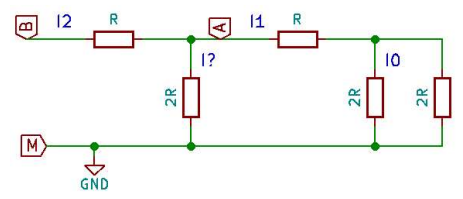
\includegraphics[width=0.5\textwidth]{images/R_2R.png}
\end{center}

\begin{enumerate}
	\item Que vaut le courant $I_1$ en fonction du courant $I_0$ (courant passant par la résistance $2R$) ?
	\item Que vaut le courant $I_2$ en fonction du courant $I_0$ (courant passant par la résistance $2R$) ?
\end{enumerate}

\textbf{Montage complet}

On s'intéresse à présent au montage suivant :

\begin{center}
	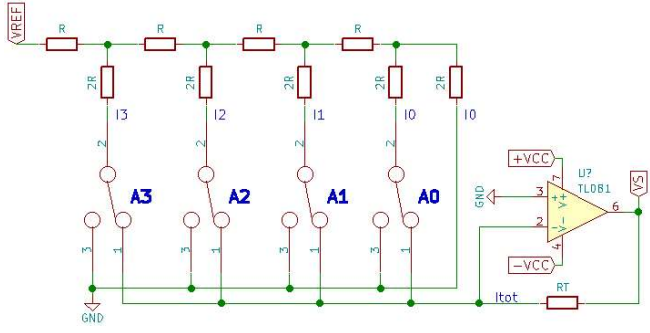
\includegraphics[width=0.8\textwidth]{images/R_2R_complet.png}
\end{center}

On supposera que lorsque $A_i = 0$, l'interrupteur $i$ est en position 3 et que lorsque Ai = 1, l'interrupteur $i$ est en position 1.

\begin{enumerate}
	\item Quel est le type de montage autour de l'ALI ?
	\item En quoi la structure vue précédemment peut nous aider ?
	\item Que vaut alors le courant $I_{tot}$ dans la contre-réaction de l'ALI en fonction des courants $I_i$ ?
	\item Que vaut alors le courant $I_{tot}$ dans la contre-réaction de l'ALI en fonction du courant $I_0$ et des
valeurs des $A_i$ ?
\end{enumerate}

\end{document} 